%%% 1 Introduction/ %%%
\chapter{Introduction} \label{ch:intro}
\begin{comment}
Some general text talking about the thesis scope in general ...
Introduction to the topic, development of the rationale,
description of the thesis’s objectives and the unfolding
structure of the chapters.\\

State the scientific problem, question, goal or hypothesis.
Outline the importance, context and relevance
\end{comment}
There are real-life problems such as the analysis and location of road accidents in a specific area that can be modified by spatial point processes,i.e., mathematical models used to describe randomly distributed events in time and space. The analysis of road accident counts can be generally done considering them to be Poisson distributed \cite{car-poisson}. In previous works, points that occur on the road network have been studied, such as, traffic accidents \cite{yamada} or wildlife-vehicle collisions \cite{borrajo}.

\section{Motivation}
    The safety regarding road vehicles is an important concern for humanity. According to \ac{WHO}, road crashes are one of the principal causes of death worldwide with almost 1.3 million \cite{who} of deaths each year. The officially reported number of COVID-19 deaths in 2020 was about 1.8 million \cite{covid} and although the numbers are not certain and \ac{WHO} estimates a higher number, it is in the same order of magnitude as road crashes fatalities.
    \\
    \\
    Furthermore, in agreement with the \ac{ERTRAC} document about Safe Road Transport Research Roadmap \cite{ertrac}, transport crashes (especially road crashes) are listed as one of the major causes of death in Europe. In its Road Safety Policy Framework 2021-2030, the European Union aims to move close to zero the number of road fatalities and injuries by the year 2050. Despite all the efforts from previous years (the European CARE database shows a 45\% reduction of road fatalities between 2000 and 2010 \cite{care}), the EU is nowadays in a situation of stagnation regarding further improvement of road safety. Although European roads are considered to be the safest roads in the world, the number of deaths each year is still disturbing.
    Statistics show \cite{ertrac} that fatalities and injuries have remained almost constant since 2014 (Figure \ref{fig:road_safety}). 
    \\
    \\
    \begin{figure}[ht] 
    \centering
    \captionsetup{justification=centering}
    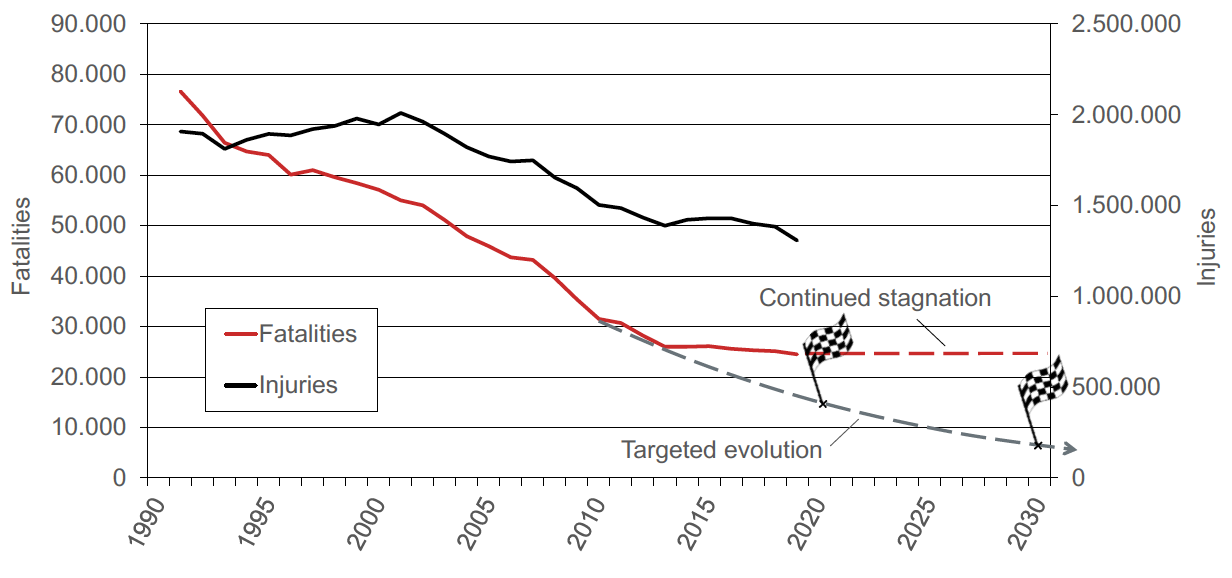
\includegraphics[width=\textwidth]{Images/Road_safety_evolution.png}
    \caption[Road safety evolution]{Road safety evolution \parencite{ertrac}.}
    \label{fig:road_safety}
    \vspace{-0.5em}
    \end{figure}
    It seems like they managed to reduce the number of deaths until 2014 but then, the vehicles' technology was safe enough and there were no more improvements to security (functional safety). Therefore, it is quite difficult for vehicle security systems (like break systems) to fail. The fatalities curve stopped decreasing, as predicted, and started to become constant. This seems to show that there is not much margin to improve safety although there is a high demand, both political and social, to approach zero deaths on the road. \\
    \\
        %TO DO: ISO 26262 , titled "Road vehicles - functional safety" is a standard whose goal is to ensure safety throughout the lifecycle of automotive equipment and systems. made a revolution but there is nothing else to improve\\
        %ISO/FDIS 21448:2022(E) Rimantas
    Human error (human limitations like the lack of reflexes, distractions, etc) is the cause of most of the accidents on roads. Thus, it comes to the stage the idea that the best way of achieving this global objective and keep improving safety is automated driving functions in fully connected vehicles and infrastructure, since this will allow the human factor to not play such an important role in driving. Giving place with these methods to safer vehicles whose driving is gradually switching control from human to machine.
    \\
    \\
    Innovation and research about autonomous driving are definitely key roles in this matter because if the human error is measured and identified, it will be possible to gradually replace it with automated techniques. In the \ac{ERTRAC} document \cite{ertrac}, it is expressed that road safety analysis is key in order to pursue road safety management. Some of the expected outcomes mentioned are "guidelines for crash data collection, open access European in-depth crash database with long-term funding concept, new data analysis methods, ...". Learning from previous accidents can be very useful to indicate which roads are safe or dangerous and under which circumstances safety can be compromised, for example, under specific weather conditions. With the research in this thesis the desire is to analyse road accidents and estimate which circumstances affect more the number of accidents, providing a measure on the safety of the roads that can be useful to quantify risk. Having this measure, it will be very beneficial for people and authorities to ask for caution and measures to warn about the possible risks on the country's road network. 
   % \\
   % TO DO: Automated cars are cheaper (it’s optimise and all automate car will be on the road and not in the garage, it will be cheaper to rent a autonomous cars by pushing a button, it will have more seats and no need to pay anyone), efficiency
    %\\
    %TO DO: Rimantas presentation about the motivation:
    %- The absence of an unreasonable level of safety risk. A criteria to quantify how safe or unsafe is a road.
    %\\
   %TO DO: Write about the importance of autonomous cars. Even remote driving can be a solution and cheap.
   %\\
    %TO DO: https://databricks.com/blog/2021/12/17/building-a-geospatial-lakehouse-part-1.html\\
    %\\
    %TO DO: https://databricks.com/blog/2022/03/28/building-a-geospatial-lakehouse-part-2.html

\section{Goal of the thesis}
The main purpose is to process the provided accident data and transform it for further analysis. In fact, using this data together with the country's map data, the goal is to construct a graph representing the road network, map the accidents on it and demonstrate that the result can be used for Poisson Regression. This way, it is possible to perform inference on the number of accidents based on different conditions to explain the frequency of accidents as a function of various factors that describe the road graph. Some questions regarding driving safety may arise when thinking about this topic: which municipalities are the most safe or dangerous, or which weather or light conditions influence more the safety on the roads. This research aims to answer such questions.
%The accidents are distributed based on the country municipalities and a discrete approach to segment the country road network is performed. together with a map matching algorithm to map the accident events on the road network and to finalize, a Poisson Regression method is applied to it.
\\
\\ 
The work in this thesis has been done in collaboration with both Uppsala University and
Sensmetry, a company that has provided data resources, expertise and financing for this research.
The data used is not publicly available and it has been accessed and provided thanks to
Sensmetry.
\section{Outline}
This chapter has introduced the motivation and goal of the thesis. Later, in Chapter \ref{ch:theory} the theory behind this research is presented. In addition, a database containing accident records for Lithuania has been provided and it is described in Chapter \ref{ch:data}. In Chapter \ref{ch:method}, the data processing is done together with a representation of the Lithuania's road network following two different approaches to segment it: by municipalities or by way or road segments. With the goal of locating the accidents on the roads, a map matching algorithm is used to distribute the accidents on the road network. The results obtained are presented in Chapter \ref{ch:results} as well as the discussion in Chapter \ref{ch:discussion}, and the conclusion and future work in Chapter \ref{ch:conclusion}.

